\section{Connection Movability Control}
{
	This involves managing the location tracking of User Equipment and managing their connections when they move between nodes. A UE will have two modes idle and connected. An idle UE will select a cell to camp on and will monitor other cells for if network conditions change this is called cell reselection. Whereas when a connected UE needs to change cell this is called Handover\cite{karandikar2017mobility}.
	\subsection{Handover}
	{
		This involves the transfer of a connection from one eNB to another. However, there are a number of different types of handover, I will go over the Coverage based handover, where a UE will move to another eNB as the service from the current node becomes unusable. When the UE detects that the signal strength is worse than the handover threshold then it starts to check for signal strength from other nodes. Note that this needs to be done before the signal drops below the minimum acceptable service quality otherwise you can have what is called Handover failure. Avoidance of handover failure can be achieved by increasing the Handover threshold meaning that it will start searching for replacement eNBs earlier, but this may reduce the quality of the replacement eNB choice, as the ideal cell for replacement is more likely to have changed since the eNB was selected. \Cref{fig:connectionHandover} shows an easy to understand visualisation of what is happening during a coverage based handover.  
		\begin{figure}
			\centering
			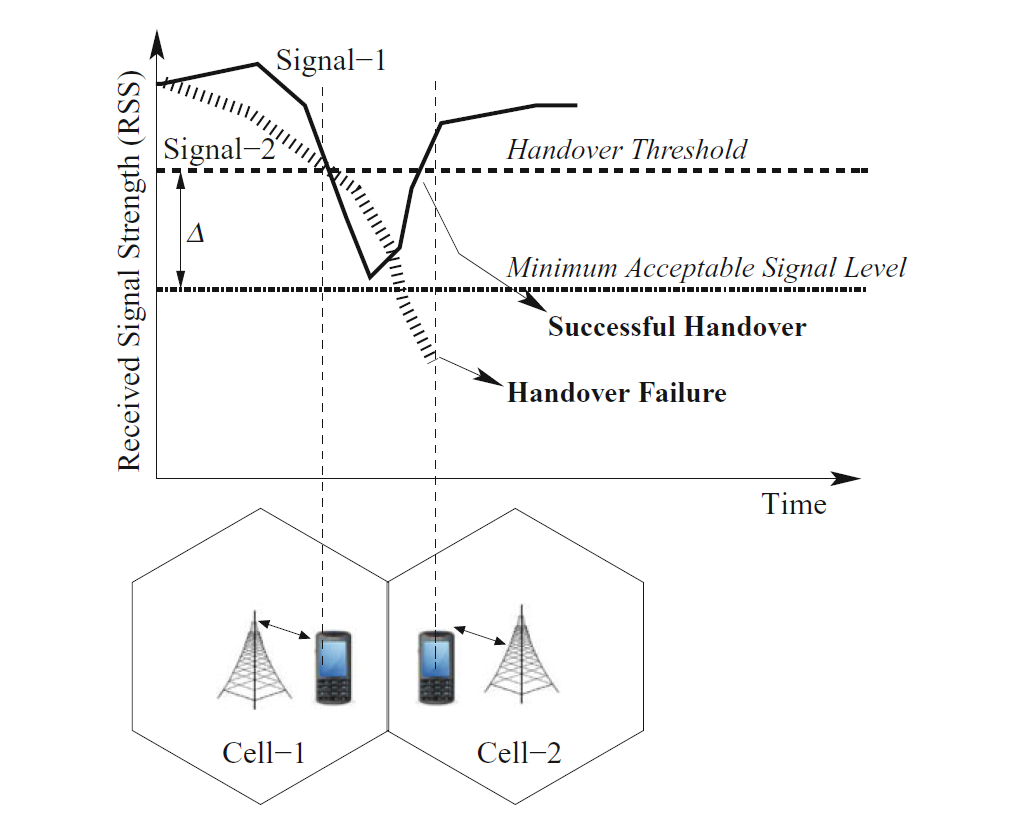
\includegraphics[width=\textwidth]{connectionHandover}
			\caption{showing how coverage-based handover occurs in LTE\cite{karandikar2017mobility}}
			\label{fig:connectionHandover}
		\end{figure}
	}
	\subsection{Cell Reselection}
	{
		This occurs when the UE is in idle mode. The UE measures the received signal from the current cells and other potential cells. The UE only switches over from one cell to another when the other cell has signal strength greater than the current cell plus some delta for a set amount of time. This avoids the problem of having the UE switch over too often when around cell edges. \Cref{fig:cellReselection} shows how the process for a UE selecting a new cell, QHysteresis is the delta which the new cells signal strength needs to be above. Treselection is the time that the new signal needs to be at least QHysteresis over the current cell signal before switching to the new cell.
		\begin{figure}
			\centering
			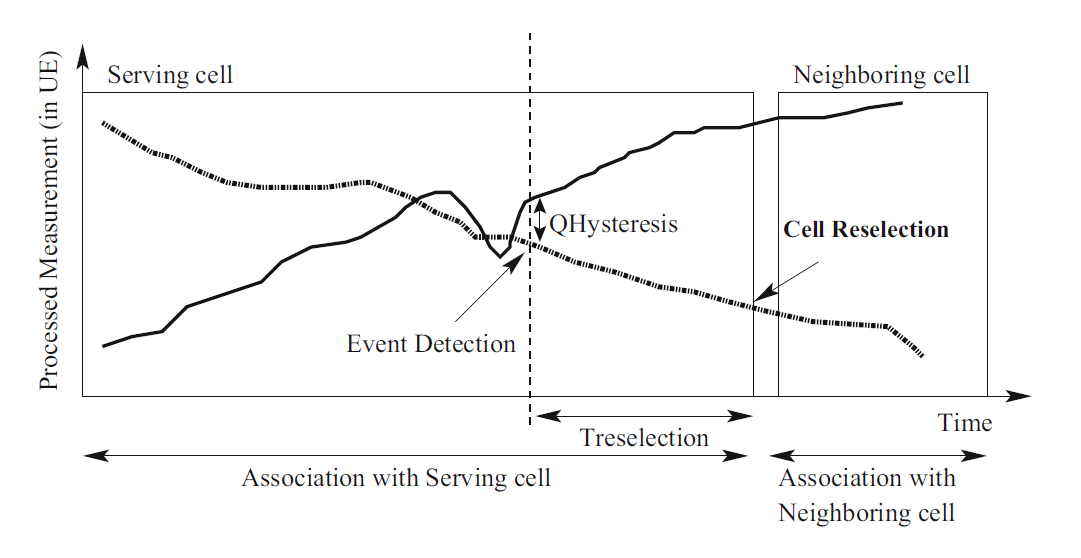
\includegraphics[width=\textwidth]{cellReselection}
			\caption{showing how cell reselection works in LTE\cite{karandikar2017mobility}}
			\label{fig:cellReselection}
		\end{figure}
	}
}